\documentclass[border=5pt]{standalone}
\usepackage[T1]{fontenc}
\usepackage{tikz}
\usetikzlibrary{positioning, arrows.meta, shapes.misc, fit, calc, backgrounds}

\definecolor{stagefill}{RGB}{232,232,232}
\definecolor{toolfill}{RGB}{255,255,255}
\definecolor{verifyfill}{RGB}{210,230,255}
\definecolor{planfill}{RGB}{255,235,210}
\definecolor{inputfill}{RGB}{240,240,250}
\definecolor{arrowgray}{RGB}{100,100,100}

\begin{document}
\sffamily
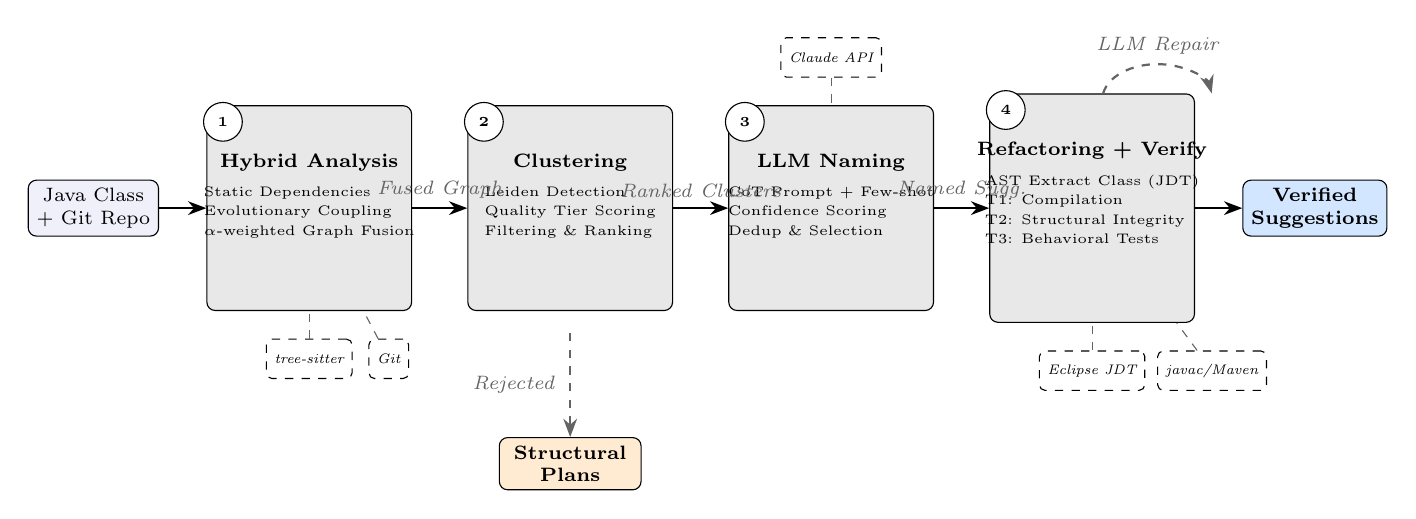
\begin{tikzpicture}[
    >=Stealth,
    stage/.style={
        draw, rounded corners=3pt, fill=stagefill,
        minimum width=2.6cm, minimum height=2.6cm,
        align=center, inner sep=4pt
    },
    tool/.style={
        draw, dashed, rounded corners=2pt, fill=toolfill,
        font=\tiny\itshape, inner sep=3pt,
        minimum height=0.5cm
    },
    output/.style={
        draw, rounded corners=3pt,
        minimum width=1.8cm, minimum height=0.6cm,
        align=center, font=\scriptsize\bfseries, inner sep=3pt
    },
    inputbox/.style={
        draw, rounded corners=3pt, fill=inputfill,
        minimum width=1.5cm, minimum height=0.6cm,
        align=center, font=\scriptsize, inner sep=3pt
    },
    flowlabel/.style={
        font=\scriptsize\itshape, text=arrowgray
    },
    stagenum/.style={
        circle, draw, fill=white, font=\tiny\bfseries,
        inner sep=1.5pt, minimum size=14pt
    },
    sublabel/.style={
        font=\tiny, align=left
    },
    every edge/.style={draw, thick, ->}
]

% ── Input ──
\node[inputbox] (input) {Java Class\\+ Git Repo};

% ── Stage 1: Hybrid Analysis ──
\node[stage, right=0.6cm of input] (s1) {};
\node[stagenum] at ([xshift=6pt, yshift=-6pt]s1.north west) {1};
\node[font=\scriptsize\bfseries, anchor=north] at ([yshift=-14pt]s1.north) {Hybrid Analysis};
\node[sublabel, anchor=north] at ([yshift=-26pt]s1.north) {%
    Static Dependencies\\[1pt]
    Evolutionary Coupling\\[1pt]
    $\alpha$-weighted Graph Fusion
};

% Stage 1 tools
\node[tool, below=0.35cm of s1] (t1a) {tree-sitter};
\node[tool, right=0.2cm of t1a] (t1b) {Git};

% ── Stage 2: Clustering ──
\node[stage, right=0.7cm of s1] (s2) {};
\node[stagenum] at ([xshift=6pt, yshift=-6pt]s2.north west) {2};
\node[font=\scriptsize\bfseries, anchor=north] at ([yshift=-14pt]s2.north) {Clustering};
\node[sublabel, anchor=north] at ([yshift=-26pt]s2.north) {%
    Leiden Detection\\[1pt]
    Quality Tier Scoring\\[1pt]
    Filtering \& Ranking
};

% ── Stage 3: LLM Naming ──
\node[stage, right=0.7cm of s2] (s3) {};
\node[stagenum] at ([xshift=6pt, yshift=-6pt]s3.north west) {3};
\node[font=\scriptsize\bfseries, anchor=north] at ([yshift=-14pt]s3.north) {LLM Naming};
\node[sublabel, anchor=north] at ([yshift=-26pt]s3.north) {%
    CoT Prompt + Few-shot\\[1pt]
    Confidence Scoring\\[1pt]
    Dedup \& Selection
};

% Stage 3 tool
\node[tool, above=0.35cm of s3] (t3) {Claude API};

% ── Stage 4: Refactoring + Verification ──
\node[stage, right=0.7cm of s3, minimum height=2.9cm] (s4) {};
\node[stagenum] at ([xshift=6pt, yshift=-6pt]s4.north west) {4};
\node[font=\scriptsize\bfseries, anchor=north] at ([yshift=-14pt]s4.north) {Refactoring + Verify};
\node[sublabel, anchor=north] at ([yshift=-26pt]s4.north) {%
    AST Extract Class (JDT)\\[1pt]
    T1: Compilation\\[1pt]
    T2: Structural Integrity\\[1pt]
    T3: Behavioral Tests
};

% Stage 4 tools
\node[tool, below=0.35cm of s4] (t4a) {Eclipse JDT};
\node[tool, right=0.15cm of t4a] (t4b) {javac/Maven};

% LLM Repair loop (dashed self-loop at top of Stage 4)
\draw[dashed, ->, thick, color=arrowgray]
    ([xshift=4pt]s4.north) arc[start angle=170, end angle=10, x radius=0.7cm, y radius=0.45cm]
    node[midway, above, font=\scriptsize\itshape, text=arrowgray] {LLM Repair};

% ── Outputs ──
\node[output, fill=verifyfill, right=0.6cm of s4] (verified) {Verified\\Suggestions};
\node[output, fill=planfill, below=1.6cm of s2] (plans) {Structural\\Plans};

% ══ ARROWS ══

% Input → Stage 1
\draw[thick, ->] (input) -- (s1);

% Stage 1 → Stage 2
\draw[thick, ->] (s1) -- node[above, flowlabel] {Fused Graph} (s2);

% Stage 2 → Stage 3 (main path)
\draw[thick, ->] (s2) -- node[above, flowlabel] {Ranked Clusters} (s3);

% Stage 2 → Structural Plans (rejected clusters, dashed)
\draw[thick, dashed, ->, color=arrowgray]
    ([yshift=-8pt]s2.south) -- node[left, flowlabel, xshift=-2pt] {Rejected} (plans);

% Stage 3 → Stage 4
\draw[thick, ->] (s3) -- node[above, flowlabel] {Named Sugg.} (s4);

% Stage 4 → Verified Suggestions
\draw[thick, ->] (s4) -- (verified);

% Stage 1 tool connections
\draw[thin, dashed, color=arrowgray] (t1a) -- (s1);
\draw[thin, dashed, color=arrowgray] (t1b) -- (s1);

% Stage 3 tool connection
\draw[thin, dashed, color=arrowgray] (t3) -- (s3);

% Stage 4 tool connections
\draw[thin, dashed, color=arrowgray] (t4a) -- (s4);
\draw[thin, dashed, color=arrowgray] (t4b) -- (s4);

\end{tikzpicture}
\end{document}
